\section{Messungen und Ergebnis}
\subsection{Grundlage}
Als Grundlage zur Bewertung von Optimierungen, soll eine \textbf{Single Page Applikation} verwendet werden. Single Page Anwendungen folgen dem Paradigma niemals die gesamte Seite neu zu laden, sondern nur gewünschte Teile der Anwendung zu aktualisieren. Oft werden dabei asynchrone Requests oder auch Web-Sockets verwendet. Dies verbessert Ladezeiten oder auch SEO. Weiterhin wird versucht ohne das Neuladen von Seiten die Web-Anwendung wie eine Desktop-Anwendung darzustellen.  

Die Messdaten basieren auf einem frei erhältlichen HTML5-Template, welches von der Seite \textit{http://egrappler.com} heruntergeladen werden kann. Die Abbildung \ref{messdaten-screenshot} zeigt einen Ausschnitt der Seite.

\begin{figure}[h!]
	\begin{center}
		
\includegraphics[width=0.9\textwidth]{img/messdaten}
		\caption{Screenshot der Messdaten}
		\label{messdaten-screenshot}	
	\end{center}
\end{figure}

Weiterhin wurde ein eigener minimalistischer Webservice, basierend auf \textit{Ruby Rack}\footnote{Ruby Rack: http://rack.github.io} und \textit{WEBrick}\footnote{WEBrick: http://www.ruby-doc.org/stdlib-2.0.0/libdoc/webrick/rdoc/index.html}, entwickelt. Der Webdienst dient zur Bereitstellung der Testdaten vor und nach der Optimierung. Das Listing \ref{server_rb} zeigt die Implementierung des Dienstes, welcher den aus der Standard-Ruby-Implementierung mitgelieferten Web-Server nutzt und auf Port 80 lauscht. 

\begin{lstlisting}[label=server_rb,language=Ruby, caption=Ruby Webservice für Messdaten]
#!/usr/bin/env ruby

# USAGE: ./server.rb path/to/the/root/dir

require 'rubygems'
require 'rack' # rack it up

serve = Rack::Builder.new do
 use Rack::Static, 
   :urls => ["/images", "/js", "/css"],
   :root => ARGV[0],
   :index => 'index.html'
 run Rack::File.new(ARGV[0])
end

# by default WEBrick doesen`t listen to sigkill, cause the script runs in a new session. 
Signal.trap('INT') {
  Rack::Handler::WEBrick.shutdown
}

# takeoff
Rack::Handler::WEBrick.run(serve, :port => 80, 'Contetn-Type'=>'text/html')
\end{lstlisting}

\subsection{Bewertung}
Das Ergebnis soll durch folgende Arten gemessen werden:
\begin{itemize}
    \item{Anzahl Dateien}
    \item{Dateigröße}
    \item{Ladezeit im Browser}
    \item{Anzahl Knoten im generierten Baum}
\end{itemize}

\begin{figure}[ht!]
	\begin{center}
		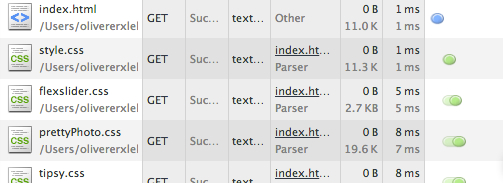
\includegraphics[width=0.9\textwidth]{img/ladezeiten_chrome_dflt}
		\caption{Ladezeiten ohne Optimierung}
		\label{ladezeiten-dflt}	
	\end{center}
\end{figure}

\begin{figure}[ht!]
	\begin{center}
		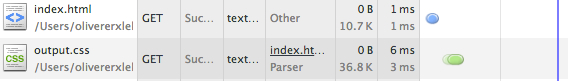
\includegraphics[width=0.9\textwidth]{img/ladezeiten_chrome_opted}
		\caption{Ladezeiten mit Optimierung}
		\label{ladezeiten-opted}	
	\end{center}
\end{figure}

Die Tabelle \ref{messungen-ergebnis} grenzt die Messergebnisse von einander ab. Nachfolgend werden die Optimierungen erläutert.

\begin{table}[ht!]
	\centering
	\begin{tabular}{l | c | c}
		Art & Ursprung & Optimierung \\
		\hline
		Anzahl Dateien & 1..n Dateien & 1 Datei \\
		Größe & ca. 37 KB & ca. 33 KB \\
		Ladezeit & 26 ms & 6 ms\\
		Anzahl Knoten im Baum & 317 & 302 \\
	\end{tabular}
	\caption{Ergebnis der Messungen}
	\label{messungen-ergebnis}
\end{table}

Die Anzahl der Dateien wird verringert. Im Beispiel der Messdaten wird aus vier CSS-Dateien eine CSS-Datei zusammengeführt. Dies verringert den Overhead für den Browser und verbessert die Ladezeiten sehr. 

Die Abbildungen \ref{ladezeiten-dflt} und \ref{ladezeiten-opted} zeigen Ausschnitte aus den Entwicklerwerkzeugen von Google Chrome. Mit diesen ist es möglich alle zu ladenden Dateien zu überwachen und mit welcher Geschwindigkeit der Browser diese lädt. Wie die Abbildungen zeigen benötigen die vier nicht optimierten Dateien aus Abbildung \ref{ladezeiten-dflt} länger als die optimierte CSS-Datei. 

Im Beispiel werden mehrere Knoten im Baum entfernt. Dies geschieht durch das Zusammenführen identischer Knoten. Außerdem wird die optimierte CSS-Datei beim Schreiben minifiziert, sodass Whitespaces und Linebreaks entfernt werden. Dies führt zur Reduktion der Ausgabedatei. 
 
\pagebreak

\subsection{Fazit}
Mittels (F)lex, Yacc/Bison und der verwendeten Grammatik kann ein Baum generiert und dessen Knoten optimiert werden. Die CSS-Dateien können mit dem entwickelten Tool Webseiten beschleunigen. Wie die Testdaten zeigen, ergibt sich eine Beschleunigung von ca. 75 \% beim Laden der CSS-Daten. 

Die Anwendung benötigt neben Flex und Yacc/Bison keine weiteren Abhängigkeiten, sodass eine gute Plattformunabhängigkeit gewährleistet ist. Der Sourcecode wurde im Rahmen der Hausarbeit unter Ubuntu 10.10, Ubuntu 12.04 mittels gcc und unter Mac OS X mittels clang und gcc erfolgreich kompiliert. 

Der vorgestellte CSS-Optimierer lässt sich für statische Websites und für Single Page Web-Apps gut einsetzen. Allerdings kann es zu Problemen kommen, wenn die Web-Anwendung eine Template-Engine einsetzt oder dynamisch CSS-Resourcen in die Seite lädt. Neue Resourcen, HTML-Elemente oder auch CSS-Stile können somit nicht optimiert werden. 

Auf CSS selbst können noch weitere Optimierungen folgen, die allerdings im Rahmen dieser Hausarbeit nicht durchgeführt wurden. 

Neben CSS sollte vor allem auch JavaScript optimiert werden, da so alle Resourcen einer Web-Anwendung verbessert werden und eine noch größere Reduktion der Ladezeiten entstehen kann. 
